\documentclass[a4paper,12pt]{article}

\usepackage[T2A]{fontenc}
\usepackage[utf8]{inputenc}
\usepackage[russian]{babel}
\usepackage{cmap}

\usepackage{amsmath,amssymb,mathtools}
\usepackage[a4paper,left=22mm,right=15mm,top=18mm,bottom=18mm]{geometry}
\usepackage{indentfirst}
\usepackage{graphicx}
\usepackage{float}
\usepackage{caption}
\usepackage{booktabs}
\usepackage{tabularx}
\usepackage{enumitem}
\usepackage{titlesec}
\usepackage[unicode,hidelinks]{hyperref}

\captionsetup{labelsep=endash,font=small,skip=4pt}
\addto\captionsrussian{\renewcommand{\figurename}{Рисунок}\renewcommand{\tablename}{Таблица}}

\titleformat{\section}{\normalfont\large\bfseries}{\thesection}{0.6em}{}
\titleformat{\subsection}{\normalfont\normalsize\bfseries}{\thesubsection}{0.6em}{}
\titlespacing*{\section}{0pt}{12pt}{5pt}
\titlespacing*{\subsection}{0pt}{9pt}{3pt}

\setlength{\parindent}{1.25cm}
\setlength{\emergencystretch}{1.5em}
\linespread{1.08}
\setlist{itemsep=1pt,topsep=3pt}

\graphicspath{{figures/}}
\newcommand{\code}[1]{\texttt{#1}}
\newcommand{\erf}{\operatorname{erf}}
\newcommand{\erfc}{\operatorname{erfc}}

\begin{document}

\begin{center}
  {\Large\bfseries Лабораторная 3: объяснение формул, параметров и программы\par}
  \vspace{4pt}
  {Уравнение теплопроводности на прямой и полупрямой\par}
\end{center}

Этот файл~--- подготовка к защите: что означает каждый параметр, откуда берётся
каждая формула, как она считается в коде и как это видно на графиках. Рисунки
строит \code{make\_figures.py}.

\tableofcontents

% ======================================================================
\section{Уравнение и его параметры}

\begin{equation}\label{eq:heat}
  u_t=a^2u_{xx}+f(x,t).
\end{equation}

\begin{table}[H]
\centering
\caption{Величины задачи и поля программы}
\begin{tabularx}{\textwidth}{@{}l l X@{}}
\toprule
Обозначение & Поле в программе & Смысл\\
\midrule
$u(x,t)$ & --- & температура стержня в точке $x$ в момент $t$ (искомая функция)\\
$a$ & \code{a} & $a^2$~--- коэффициент температуропроводности $a^2=k/(c\rho)$
($k$~--- теплопроводность, $c$~--- теплоёмкость, $\rho$~--- плотность). Чем больше $a$,
тем быстрее выравнивается температура. Характерная ширина «размытия» за время $t$~--- $2a\sqrt t$\\
$\varphi(x)$ & $\varphi(x)$ & начальная температура $u(x,0)$\\
$f(x,t)$ & \code{f(x,t)} & плотность источников тепла (делённая на $c\rho$): $f>0$~--- нагрев, $f<0$~--- охлаждение\\
$\mu(t),\nu(t)$ & $\mu(t)$, $\nu(t)$ & задание Б: их произведение~--- правая часть
граничного условия $u_x(0,t)=\mu(t)\nu(t)$\\
род условия & \code{граничное условие} & 2~--- $u_x(0,t)=\mu\nu$ (вариант группы, задан поток);
1~--- $u(0,t)=\mu\nu$ (задана температура конца)\\
способ & \code{способ} & задание А: \code{poisson}~--- формула Пуассона~\eqref{eq:poisson},
\code{green}~--- свёртка с функцией Грина на сетке~\eqref{eq:greengrid}\\
$T$ & \code{длительность T} & отрезок времени $[0,T]$ анимации\\
$x_{\min},x_{\max}$ & \code{границы x} & окно графика (на решение не влияют: задача на всей прямой/полупрямой)\\
$\xi_0$ & «$\xi_0$ для графика $G$» & точка источника, для которой рисуется функция Грина $G(x,\xi_0,t)$\\
кадров & \code{кадров} & число моментов $t_k=kT/(N-1)$, в которые считается решение\\
скорость & \code{мс/кадр} & пауза между кадрами анимации (только показ)\\
\bottomrule
\end{tabularx}
\end{table}

Уравнение~\eqref{eq:heat} следует из закона Фурье (поток тепла $q=-k\,u_x$)
и баланса энергии на отрезке $[x,x+dx]$:
$c\rho\,u_t\,dx=\bigl(q(x)-q(x+dx)\bigr)+F\,dx$, откуда $c\rho\,u_t=k\,u_{xx}+F$.
Делим на $c\rho$: $a^2=k/(c\rho)$, $f=F/(c\rho)$.

Знак $u_x$ на границе: поток в сторону $+x$ равен $q=-k\,u_x$. Поэтому при
$u_x(0,t)<0$ поток направлен внутрь стержня (тепло входит), при $u_x(0,t)>0$~---
наружу, $u_x(0,t)=0$~--- теплоизоляция.

% ======================================================================
\section{Фундаментальное решение (функция Грина на прямой)}

\begin{equation}\label{eq:K}
  G(x,\xi,t)=\frac{1}{2a\sqrt{\pi t}}\exp\!\left(-\frac{(x-\xi)^2}{4a^2t}\right),\quad t>0.
\end{equation}
\textbf{Смысл.} Температура в точке $x$ в момент $t$, если в момент $t=0$
в точку $\xi$ мгновенно внесли единицу тепла: $G(x,\xi,0)=\delta(x-\xi)$.

\textbf{Свойства} (проверяются тестами \code{TestKernel}):
\begin{enumerate}
  \item $G_t=a^2G_{xx}$ при $t>0$~--- проверяется подстановкой;
  \item $\int_{-\infty}^{\infty}G\,d\xi=1$ при любом $t>0$: тепло сохраняется.
        Это интеграл Пуассона $\int e^{-z^2}dz=\sqrt\pi$ после замены $z=(x-\xi)/(2a\sqrt t)$;
  \item ширина колокола $\sim2a\sqrt t$, высота $1/(2a\sqrt{\pi t})$: при $t\to0$
        колокол сужается и растёт~--- стремится к $\delta$-функции;
  \item $G>0$ при всех $x$ и $t>0$: тепло «чувствуется» сразу везде
        (бесконечная скорость распространения~--- особенность модели, в отличие от
        волнового уравнения).
\end{enumerate}

\begin{figure}[H]
\centering
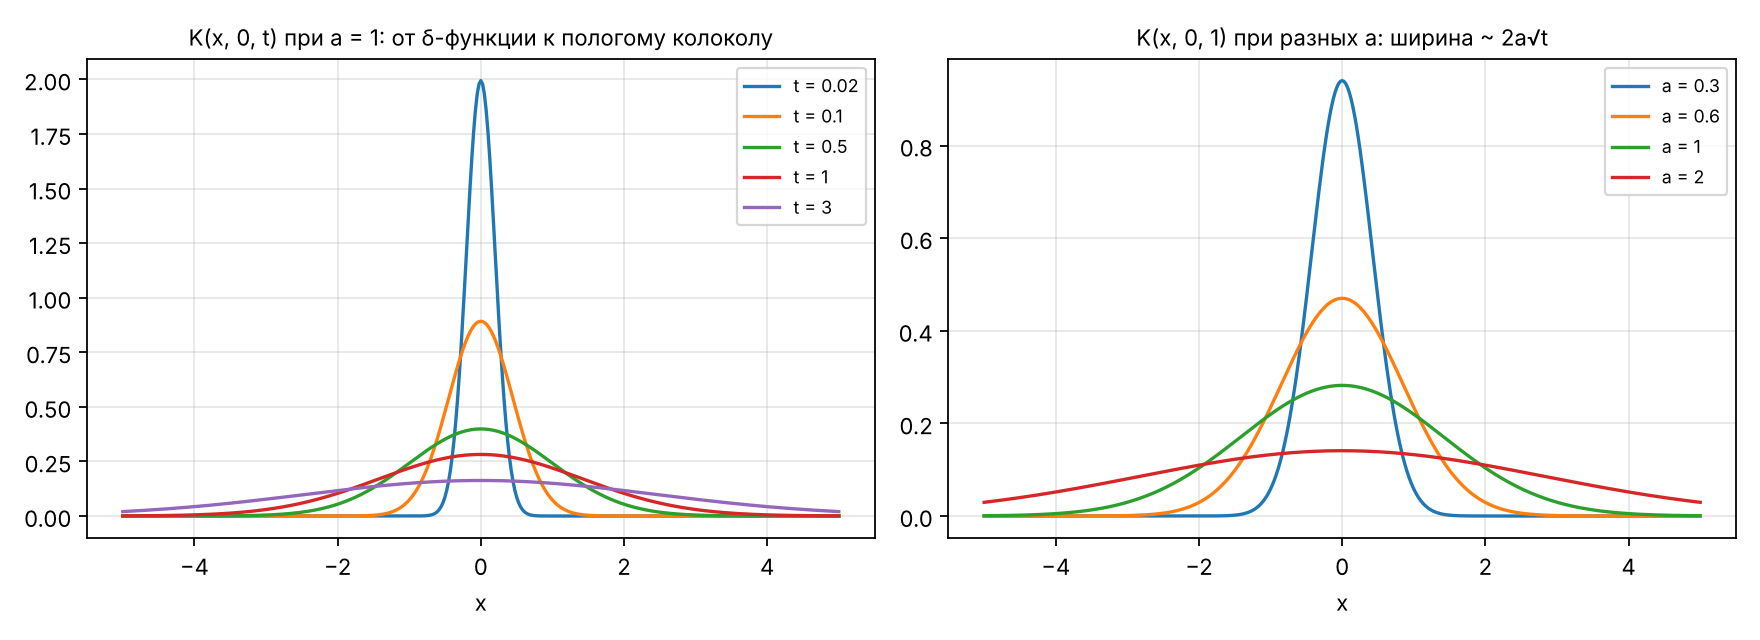
\includegraphics[width=\textwidth]{e_kernel.png}
\caption{Слева: $G(x,0,t)$ при разных $t$; справа: при разных $a$ в момент $t=1$}
\end{figure}

В коде: \code{heatlab/kernels.py}, функция \code{heat\_kernel(x, xi, t, a)};
при $t\le0$ возвращается 0 (дельта-функцию нельзя записать числом~--- при $t=0$
программа выдаёт $\varphi(x)$ напрямую), при показателе $>700$~--- тоже 0
(чтобы \code{exp} не уходил в машинный нуль с потерей точности).

% ======================================================================
\section{Задание А}

\subsection{Формула решения}
\begin{equation}\label{eq:solA}
  u(x,t)=\underbrace{\int_{-\infty}^{\infty}G(x,\xi,t)\varphi(\xi)\,d\xi}_{\text{начальное условие}}
  +\underbrace{\int_{0}^{t}\!d\tau\!\int_{-\infty}^{\infty}G(x,\xi,t-\tau)f(\xi,\tau)\,d\xi}_{\text{источник (интеграл Дюамеля)}} .
\end{equation}
\textbf{Почему так.} Уравнение линейно, поэтому решение~--- сумма откликов
на отдельные «кусочки» данных. Начальная температура~--- набор точечных источников
$\varphi(\xi)\,d\xi$ в момент 0; каждый даёт $G(x,\xi,t)\varphi(\xi)d\xi$.
Источник $f$ за время $d\tau$ вносит тепло $f(\xi,\tau)d\xi\,d\tau$ в момент $\tau$,
к моменту $t$ оно расплывается как $G(x,\xi,t-\tau)$. Это и есть принцип
Дюамеля. На рис.~\ref{fig:superpos} справа видно, что $u(0,t)$ для
$\varphi$ и $f$ вместе равно сумме двух отдельных решений.

\subsection{Способ 1: формула Пуассона}
После замены $\xi=x+2a\sqrt t\,z$ ($d\xi=2a\sqrt t\,dz$):
\begin{equation}\label{eq:poisson}
  \int G\varphi\,d\xi=\frac{1}{\sqrt\pi}\int_{-\infty}^{\infty}\varphi\bigl(x+2a\sqrt t\,z\bigr)e^{-z^2}dz .
\end{equation}
\textbf{Смысл:} $u(x,t)$~--- взвешенное среднее значений $\varphi$ около $x$,
вес~--- гауссов колокол $e^{-z^2}/\sqrt\pi$ (его площадь 1), а радиус
усреднения $2a\sqrt t$ растёт со временем (рис.~\ref{fig:poisson}).

\begin{figure}[H]
\centering
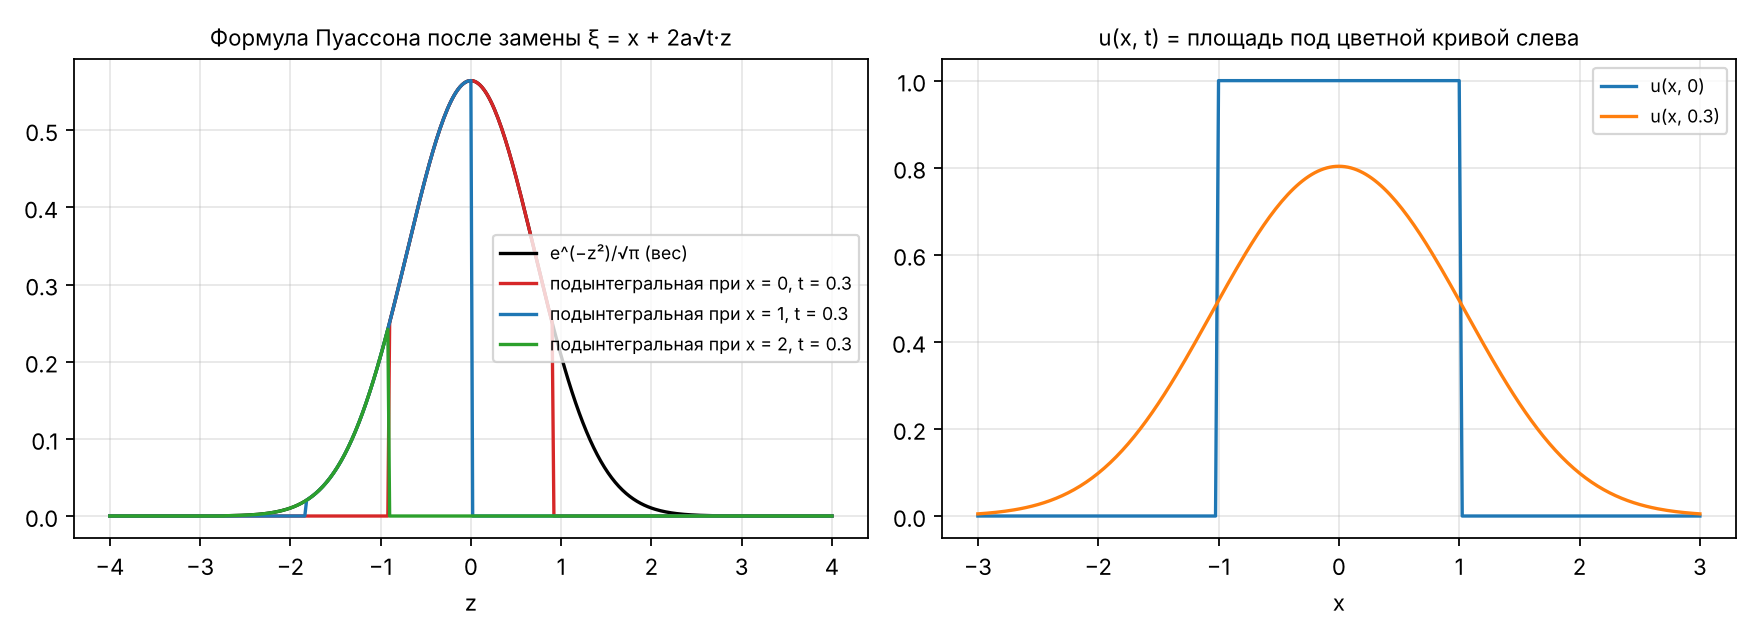
\includegraphics[width=\textwidth]{e_poisson.png}
\caption{Подынтегральная функция~\eqref{eq:poisson} для $\varphi=\theta(1-|x|)$, $t=0{,}3$
в точках $x=0,1,2$; площадь под каждой цветной кривой~--- значение $u(x,0{,}3)$ справа}
\label{fig:poisson}
\end{figure}

\textbf{Как считается.} Интеграл обрезается до $|z|\le Z=6$ ($e^{-36}\approx
2\cdot10^{-16}$~--- меньше машинной точности) и берётся адаптивной формулой
Симпсона (\code{numint.adaptive\_simpson}):
\begin{itemize}
  \item отрезок $[-6,6]$ режется на 16 частей; на каждой части $[\alpha,\beta]$
        считается формула Симпсона $S=\frac{\beta-\alpha}{6}\bigl(g_\alpha+4g_m+g_\beta\bigr)$;
  \item часть делится пополам, считаются $S_{\text{лев}}$, $S_{\text{прав}}$;
        если $|S_{\text{лев}}+S_{\text{прав}}-S|\le15\varepsilon$ (оценка Рунге, у Симпсона
        ошибка $\sim h^4$, поэтому $2^4-1=15$)~--- принимаем $S_{\text{лев}}+S_{\text{прав}}+\frac{\text{разность}}{15}$,
        иначе делим дальше с допуском $\varepsilon/2$;
  \item допуск \code{tol} $=10^{-6}$. Около разрывов $\varphi$ шаг мельчает
        автоматически, на гладких участках остаётся крупным.
\end{itemize}

\subsection{Способ 2: свёртка с функцией Грина на сетке}
\begin{equation}\label{eq:greengrid}
  u(x,t)\approx\frac{\sum_j G(x,\xi_j,t)\,\varphi(\xi_j)}{\sum_j G(x,\xi_j,t)},\qquad
  \xi_j=\Bigl(j+\frac12\Bigr)h,\quad h=0{,}04,\quad |x-\xi_j|\le5\cdot2a\sqrt t .
\end{equation}
\begin{itemize}
  \item это формула средних прямоугольников $\int g\,d\xi\approx\sum g(\xi_j)h$
        для~\eqref{eq:solA} на неподвижной сетке середин ячеек $[jh,(j+1)h]$;
        множитель $h$ сокращается;
  \item знаменатель $\sum_jG(x,\xi_j,t)h\approx\int G\,d\xi=1$. Деление на него
        сохраняет «полное тепло» и при малых $t$, когда ядро уже нескольких шагов сетки;
  \item окно $|x-\xi|\le5\cdot2a\sqrt t$ ($e^{-25}\approx10^{-11}$): дальше
        вклад ничтожен; значения $\varphi(\xi_j)$ запоминаются (\code{table}) и
        не пересчитываются на следующих кадрах;
  \item для гладкой $\varphi$ ошибка $\sim10^{-12}$ (на гауссе сумма по сетке
        сходится очень быстро); при разрыве $\varphi$ в точке $c$ ошибка
        $\approx G\cdot\operatorname{dist}(c,\text{граница ячейки})\le G h/2$
        (рис.~\ref{fig:error}); если $c$ кратно $h$ (типичные $\theta(x)$,
        $\theta(1-|x|)$), ошибка $O(h^2)$.
\end{itemize}

\begin{figure}[H]
\centering
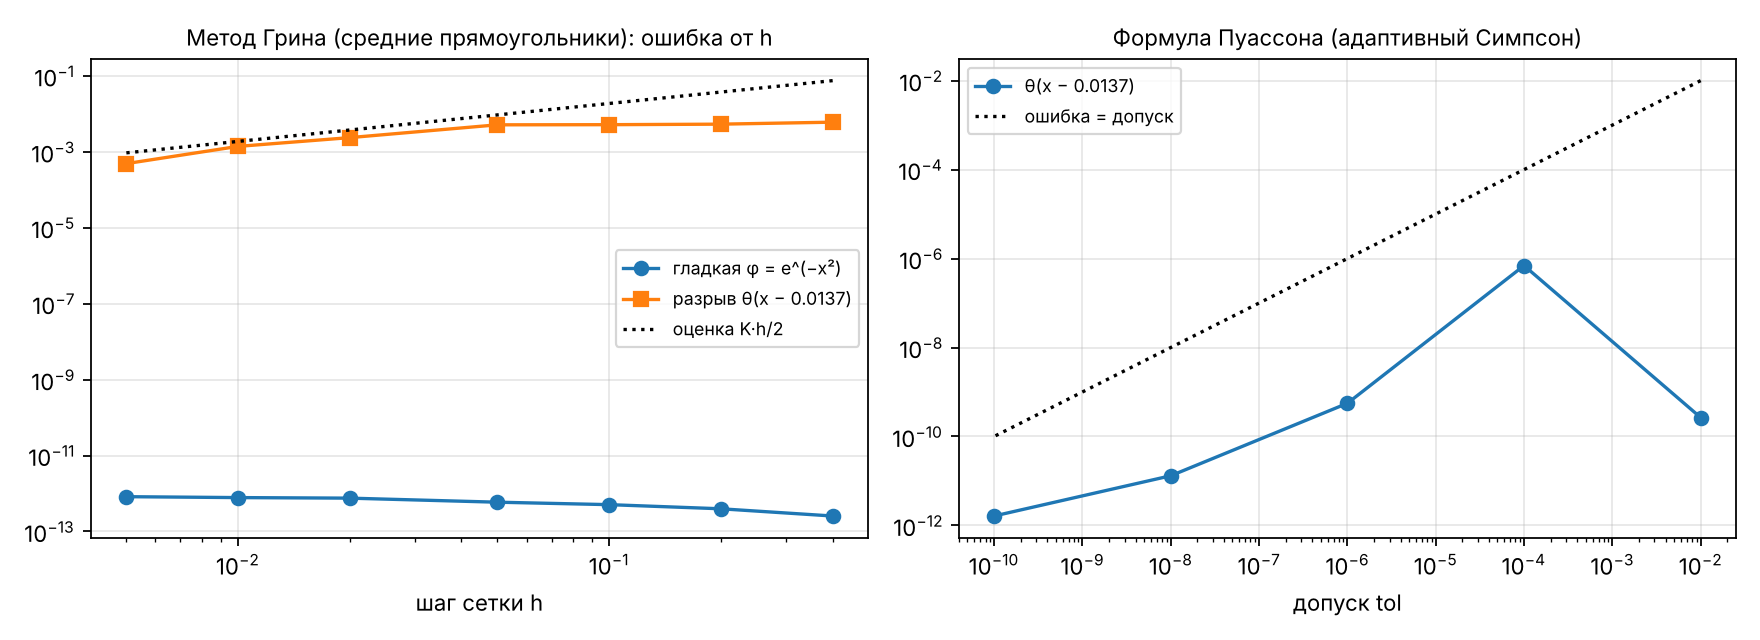
\includegraphics[width=\textwidth]{e_error.png}
\caption{Точность двух способов: слева~--- метод Грина в зависимости от шага $h$;
справа~--- формула Пуассона в зависимости от допуска адаптивного Симпсона}
\label{fig:error}
\end{figure}

\subsection{Источник $f$}
Внутренний интеграл~\eqref{eq:solA} при фиксированном $\tau$~--- та же
свёртка, но со временем $s=t-\tau$; внешний по $\tau\in[0,t]$~--- обычная
формула Симпсона с 21 узлом (\code{ntau}). Внутренний~--- Симпсон с 41 узлом
(\code{nzf}) по $z$ или сетка~\eqref{eq:greengrid}. При $\tau=t$ ($s=0$)
внутренний интеграл равен $f(x,t)$: ядро превращается в $\delta$-функцию~---
в коде \code{convolve} возвращает \code{g(x)} при $s\le0$.

\begin{figure}[H]
\centering
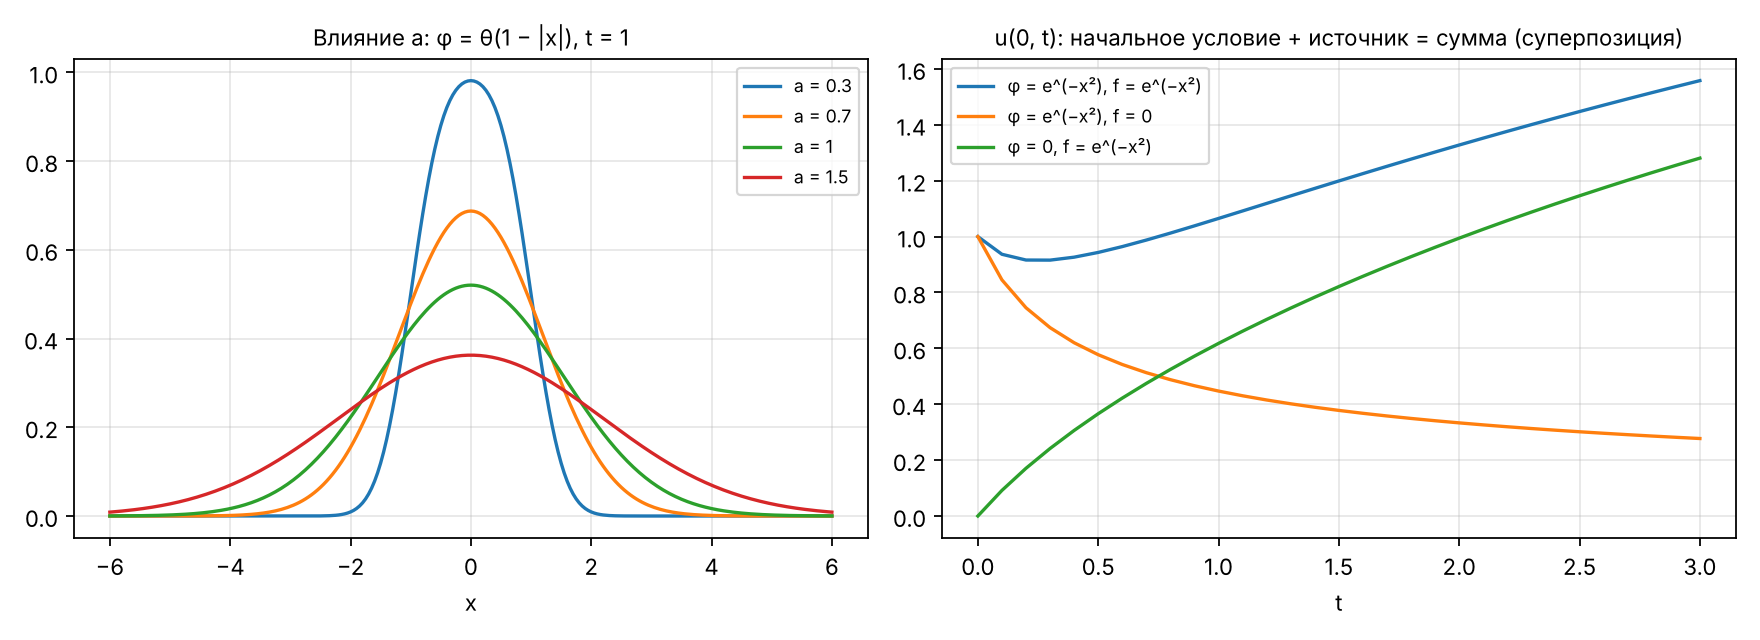
\includegraphics[width=\textwidth]{e_a_effect.png}
\caption{Слева: влияние $a$~--- чем больше $a$, тем сильнее размыт импульс к $t=1$;
справа: суперпозиция решений (начальное условие + источник)}
\label{fig:superpos}
\end{figure}

\subsection{Что видно на графике задания А}
\begin{itemize}
  \item серый пунктир~--- $\varphi(x)$, красная линия~--- $u(x,t_k)$;
  \item в заголовке~--- $\int u\,dx$ по окну графика: при $f=0$ она не меняется
        (сохранение тепла), пока «хвосты» не вышли за окно;
  \item нижний график~--- $G(x,\xi_0,t_k)$: как расплывается тепло от точечного
        источника; при $t=0$ это $\delta$-функция (подпись на графике);
  \item максимум $u$ не растёт при $f=0$ (принцип максимума), углы разрывов
        сглаживаются мгновенно.
\end{itemize}

% ======================================================================
\section{Задание Б}

\subsection{Почему отражения}
На полупрямой нужна функция Грина, которая сама удовлетворяет однородному
граничному условию. Для $u_x(0,t)=0$ (II рода) к источнику в $\xi$ добавляем
такой же в $-\xi$: сумма чётна по $x$, её производная в нуле равна 0. Для
$u(0,t)=0$ (I рода) отражённый источник берётся с минусом: разность нечётна,
в нуле равна 0.
\begin{equation}\label{eq:G12}
  G_2=G(x,\xi,t)+G(x,-\xi,t),\qquad G_1=G(x,\xi,t)-G(x,-\xi,t).
\end{equation}

\begin{figure}[H]
\centering
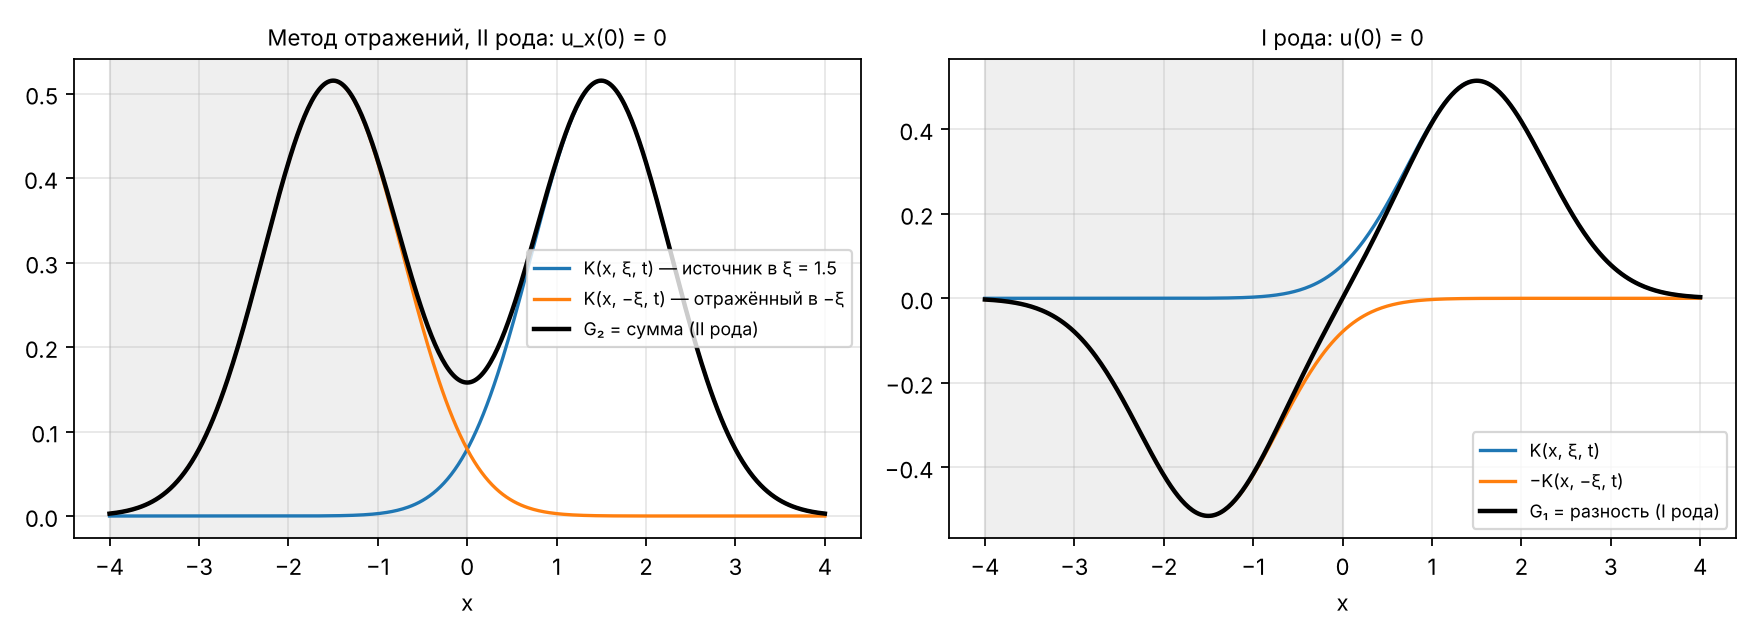
\includegraphics[width=\textwidth]{e_images.png}
\caption{Метод отражений: серым~--- «фиктивная» область $x<0$}
\end{figure}

\begin{figure}[H]
\centering
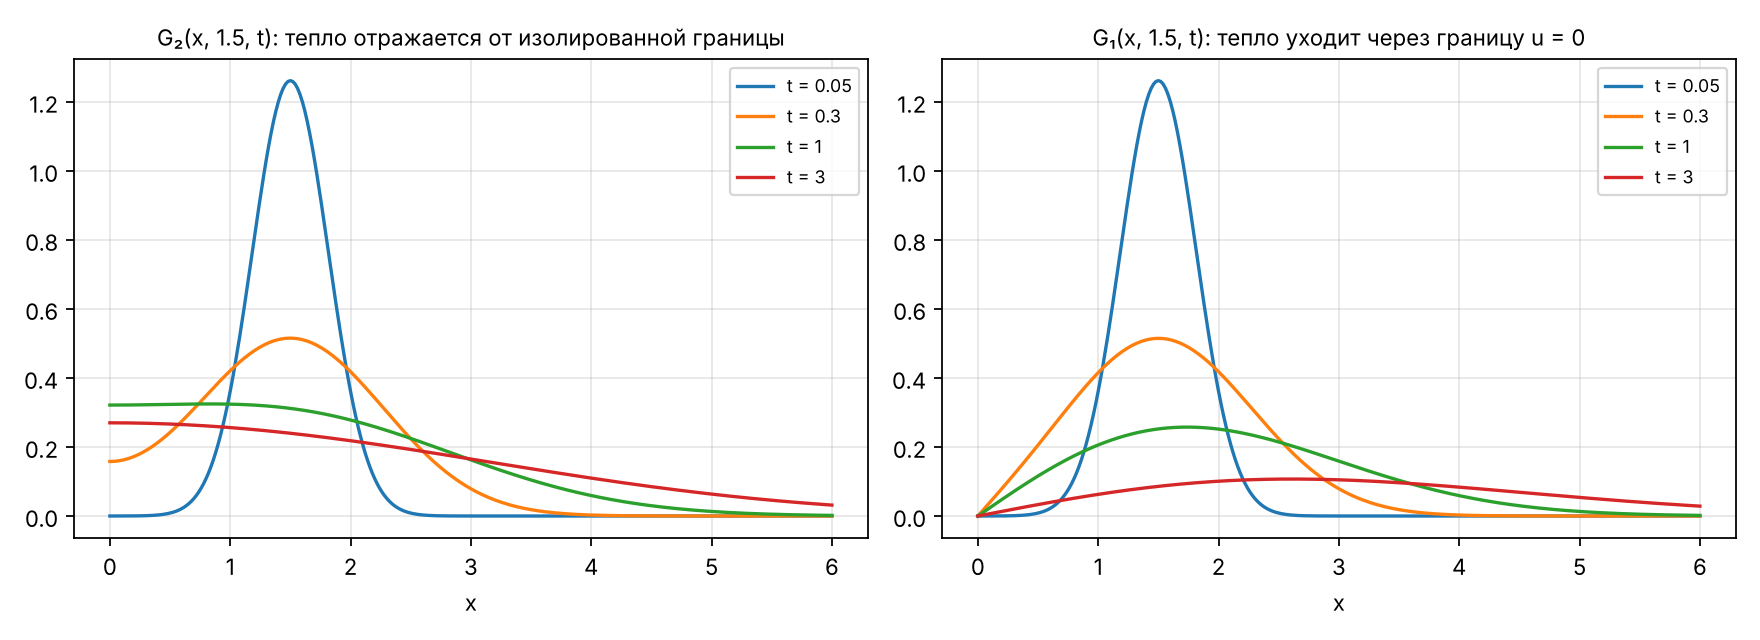
\includegraphics[width=\textwidth]{e_green_half.png}
\caption{$G_2$ и $G_1$ при $\xi=1{,}5$: изолированная граница отражает тепло
(максимум смещается к границе), граница с $u=0$ поглощает его}
\end{figure}

\subsection{Формула решения для варианта $u_x(0,t)=\mu(t)\nu(t)$}
Обозначим $g(t)=\mu(t)\nu(t)$ (в коде \code{self.g}). Формула Грина
(умножаем уравнение на $G_2(x,\xi,t-\tau)$ и интегрируем по частям по
$\xi\in(0,\infty)$, $\tau\in(0,t)$; граничный член при $\xi=0$ даёт поток):
\begin{equation}\label{eq:solB}
  u(x,t)=\underbrace{\int_0^\infty G_2(x,\xi,t)\varphi(\xi)\,d\xi}_{\code{initial\_part}}
   \;\underbrace{-\,a^2\!\int_0^t G_2(x,0,t-\tau)\,g(\tau)\,d\tau}_{\code{boundary\_part}}
   +\underbrace{\int_0^t\!\!d\tau\!\int_0^\infty G_2(x,\xi,t-\tau)f(\xi,\tau)\,d\xi}_{\code{source\_part}} .
\end{equation}
\textbf{Знак второго слагаемого.} При постоянном $g=-q<0$ (приток) и $x=0$:
$-a^2\int_0^t\frac{-q}{a\sqrt{\pi(t-\tau)}}d\tau=2aq\sqrt{t/\pi}>0$~--- граница
нагревается, как и должно быть.

\textbf{Особенность и замена.} $G_2(x,0,s)=\frac{2}{2a\sqrt{\pi s}}e^{-x^2/(4a^2s)}$:
при $x=0$ и $s\to0$ растёт как $1/\sqrt s$. Интеграл сходится, но формула Симпсона
на нём теряет точность (в узле $\tau=t$ бесконечность). Замена $t-\tau=\sigma^2$,
$d\tau=-2\sigma\,d\sigma$, $1/\sqrt{t-\tau}=1/\sigma$:
\begin{equation}\label{eq:bnd}
  -a^2\!\int_0^tG_2(x,0,t-\tau)g(\tau)\,d\tau=
  -\frac{2a}{\sqrt\pi}\int_0^{\sqrt t}g\bigl(t-\sigma^2\bigr)e^{-x^2/(4a^2\sigma^2)}\,d\sigma .
\end{equation}
Подынтегральная функция ограничена (при $\sigma=0$ она равна $g(t)$, если $x=0$,
и 0, если $x>0$), интеграл берётся адаптивным Симпсоном.

\textbf{Первое слагаемое.} Интегрируем по $\xi\in[\max(0,x-W),x+W]$,
$W=6\cdot2a\sqrt t$: вне этого отрезка и $G(x,\xi,t)$, и отражённая часть
$G(x,-\xi,t)$ меньше $10^{-16}$.

\textbf{Источник}~--- как в задании А, но внутренний интеграл с $G_2$ по $\xi>0$.

\begin{figure}[H]
\centering
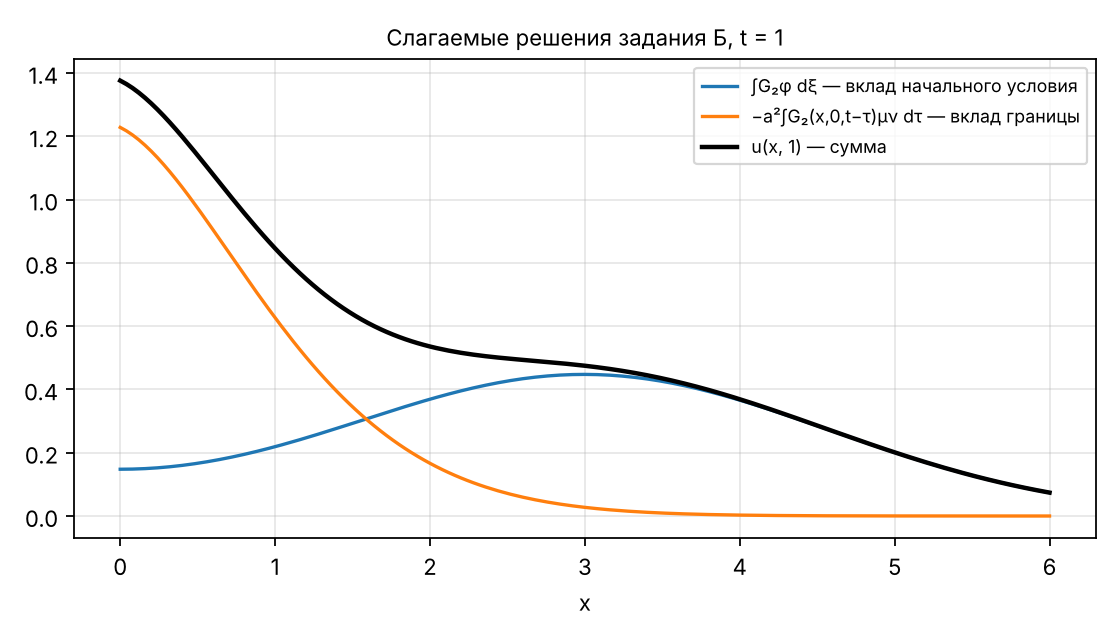
\includegraphics[width=0.75\textwidth]{e_parts.png}
\caption{Слагаемые~\eqref{eq:solB} при $t=1$: начальное условие и вклад границы}
\end{figure}

\subsection{Роль $\mu(t)$ и $\nu(t)$}
В условии варианта поток задан произведением. Удобно читать так: $\mu$~---
амплитуда (знак задаёт направление: $\mu<0$~--- нагрев через границу),
$\nu$~--- закон изменения во времени. Программе важно только произведение
$g=\mu\nu$; если одна из функций тождественно 0, граничный интеграл не считается.

\begin{figure}[H]
\centering
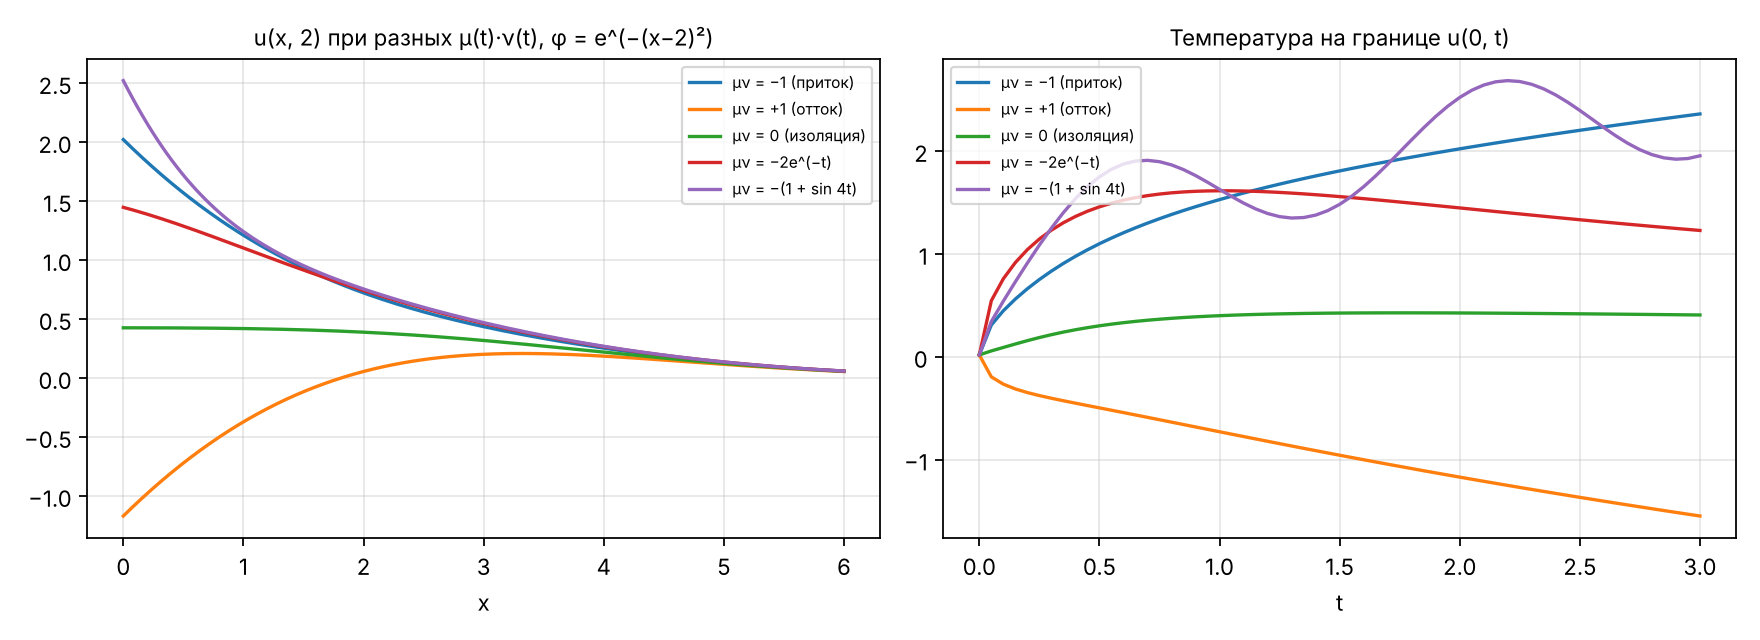
\includegraphics[width=\textwidth]{e_mu_nu.png}
\caption{Влияние $\mu\nu$: решение при $t=2$ и температура на границе $u(0,t)$}
\end{figure}

\subsection{Условие I рода (дополнительно)}
$u(0,t)=g(t)$, функция Грина $G_1$. Граничное слагаемое
$a^2\int_0^t\partial_\xi G_1(x,0,t-\tau)\,g(\tau)\,d\tau$, где
$a^2\partial_\xi G_1(x,0,s)=\frac{x}{2a\sqrt\pi\,s^{3/2}}e^{-x^2/(4a^2s)}$.
Замена $w=\frac{x}{2a\sqrt{t-\tau}}$ даёт
\[
  \frac{2}{\sqrt\pi}\int_{x/(2a\sqrt t)}^{\infty}g\!\left(t-\frac{x^2}{4a^2w^2}\right)e^{-w^2}dw ,
\]
при $x=0$ это $\frac{2}{\sqrt\pi}\int_0^\infty g(t)e^{-w^2}dw=g(t)$~--- граничное условие выполнено.

\subsection{Что видно на графике задания Б}
Сверху~--- $u(x,t_k)$ и $\varphi$; слева внизу~--- $G_2(x,\xi_0,t_k)$ (или $G_1$);
справа внизу~--- $g(t)=\mu(t)\nu(t)$ на всём $[0,T]$, точка~--- текущий момент.
Наклон $u$ у левого края графика равен текущему значению $g$.

\textbf{Согласование данных.} Если $\varphi'(0)\ne g(0)$, при $t\to0$ у границы
образуется тонкий пограничный слой~--- это свойство задачи, не ошибка расчёта:
через короткое время наклон $u$ у границы становится равным $g(t)$
(рис.~2 отчёта, справа).

% ======================================================================
\section{Проверка (тесты)}

\begin{table}[H]
\centering
\caption{Точные решения, с которыми сравнивается программа}
\begin{tabularx}{\textwidth}{@{}l X@{}}
\toprule
Данные & Точное решение\\
\midrule
$\varphi=e^{-x^2}$ & $\dfrac{1}{\sqrt{1+4a^2t}}\exp\!\left(-\dfrac{x^2}{1+4a^2t}\right)$\\
$\varphi=\theta(x)$ & $\frac12\bigl(1+\erf\frac{x}{2a\sqrt t}\bigr)$\\
$\varphi=\sin kx$ / $\cos kx$ & $e^{-a^2k^2t}\sin kx$ / $e^{-a^2k^2t}\cos kx$ (последнее~--- и на полупрямой с изоляцией)\\
$\varphi=x^2$ & $x^2+2a^2t$\\
$f=1$, $\varphi=0$ & $t$\\
Б: $\varphi=0$, $u_x(0,t)=-q$ & $2q\Bigl[a\sqrt{t/\pi}\,e^{-z^2}-\frac{x}{2}\erfc z\Bigr]$, $z=\frac{x}{2a\sqrt t}$\\
Б, I рода: $u(0,t)=1$ & $\erfc\frac{x}{2a\sqrt t}$\\
\bottomrule
\end{tabularx}
\end{table}
Функции $\erf$, $\erfc$ используются только в тестах для сравнения,
в расчётах их нет.

% ======================================================================
\section{Устройство кода}

\begin{table}[H]
\centering
\begin{tabularx}{\textwidth}{@{}l X@{}}
\toprule
Файл & Что делает\\
\midrule
\code{heatlab/numint.py} & сетка \code{linspace}, Симпсон \code{Simpson(n)}, адаптивный \code{adaptive\_simpson}, \code{trapezoid}\\
\code{heatlab/kernels.py} & $G$~\eqref{eq:K}, $G_1$, $G_2$~\eqref{eq:G12}\\
\code{heatlab/line.py} & задание А: \code{HeatLine.u}, \code{convolve} (два способа), \code{source\_part}\\
\code{heatlab/halfline.py} & задание Б: \code{HeatHalfLine.u} = \code{initial\_part} + \code{boundary\_part} + \code{source\_part}\\
\code{heatlab/userfunc.py} & строка пользователя $\to$ функция (\code{exp}, \code{sin}, \code{theta}, \dots)\\
\code{heatlab/plots.py} & рисование кадров (общее для окна, скриптов и GIF)\\
\code{task\_a.py}, \code{task\_b.py} & ввод данных, расчёт кадров, анимация, GIF\\
\code{app.py} & оконное приложение; расчёт идёт в отдельном потоке, окно не замирает\\
\code{tests/} & 23 теста\\
\bottomrule
\end{tabularx}
\end{table}

\textbf{Типичные вопросы на защите.}
\begin{itemize}
  \item \emph{Почему при $t=0$ отдельная ветка?} $G$ при $t=0$~--- $\delta$-функция,
        численно её нет; по определению $u(x,0)=\varphi(x)$.
  \item \emph{Почему обрезка $|z|\le6$?} $e^{-36}\approx2\cdot10^{-16}$~--- вклад
        хвоста меньше погрешности чисел с плавающей точкой.
  \item \emph{Чем отличаются способы А?} Пуассон~--- переменная $z$, узлы
        движутся вместе с $x$, адаптивный шаг. Грин~--- неподвижная сетка по $\xi$,
        одна таблица $\varphi(\xi_j)$ на все кадры, точность задаётся шагом $h$.
  \item \emph{Зачем замена $t-\tau=\sigma^2$?} Убирает особенность $1/\sqrt{t-\tau}$
        функции Грина у граничного интеграла.
  \item \emph{Почему решение сразу ненулевое далеко от источника?} $G>0$ при всех $x$~---
        в модели Фурье скорость распространения тепла бесконечна.
\end{itemize}

\end{document}
